\documentclass[12pt, a4paper]{report}
\usepackage[utf8]{inputenc}
\usepackage[T1]{fontenc}
\usepackage[utf8]{inputenc}
\usepackage{geometry}
\usepackage{listings}
\usepackage{xcolor}
\usepackage[]{graphicx}
\usepackage[export]{adjustbox}
\usepackage{subcaption}
\makeatletter
\setlength{\@fptop}{0pt}
\makeatother

\definecolor{codegreen}{rgb}{0.26, 0.61, 0}
\definecolor{codegray}{rgb}{0.5,0.5,5}
\definecolor{codepurple}{rgb}{58,0,0.82}
\definecolor{backcolour}{rgb}{0.80, 0.81, 0.93}

\lstdefinestyle{mystyle}{
    backgroundcolor=\color{backcolour},   
    commentstyle=\color{codegreen},
    keywordstyle=\color{magenta},
    numberstyle=\tiny\color{codegray},
    stringstyle=\color{codepurple},
    basicstyle=\ttfamily\footnotesize,
    breakatwhitespace=false,         
    breaklines=true,                 
    captionpos=b,                    
    keepspaces=true,                 
    numbers=left,                    
    numbersep=5pt,                  
    showspaces=false,                
    showstringspaces=false,
    showtabs=false,                  
    tabsize=2
}

\lstset{style=mystyle}


\title{\textbf{EE2703: Applied Programming Lab\\Assignment 5\\The Resistor Problem
}}


\author{Devaganthan S S\\ EE19B018}
\date{\today}
\begin{document}

\maketitle


\section{Abstract}
This Assignment aims to 
\begin{itemize}
  \item Solve current in a resistor using python
  \item Learn to plot Quiver, 3D, and Contour Plot.
\end{itemize}


\section{Introduction}
We have a metal plate. A circular electrode (of 1V) is placed at the center of the metal Plate. The bottom of the Metal plate is grounded. We find the potential of the plate using Laplace Equation and with the given boundary conditions. We plot the Contour, 3D plot of the Potential Function. We find the Current in the Metal, and plot the quiver plot for the same. We also find the Error in the potential after each Iteration and then plot the $loglog$ and $semilog$ plots.
\section{Results and Implementation}
\subsection{Solving and Contour and 3D Plotting for the Potential.}
We assume the Metal Plate as a grid having NX rows and NY Columns. We find points that lie within a circular region of given radius using {\fontfamily{cmss}\selectfont
'where()'
}. We perform Niter Iterations and in each iteration, we perform the following actions, Copy the Potential Matrix to a New matrix, Update the Phi Matrix, Assert Boundary Conditions, And compute the error. In the end, we have a good approximation of the Potential Function. We then plot the contour plot of the Potential Function. We plot the Contour and 3D plot of the Potential Function. The Below code Performs the above tasks.
\noindent
\lstinputlisting[language = python]{code1.py}
\begin{figure}[h!]

\begin{subfigure}{0.55\textwidth}
    \centering
    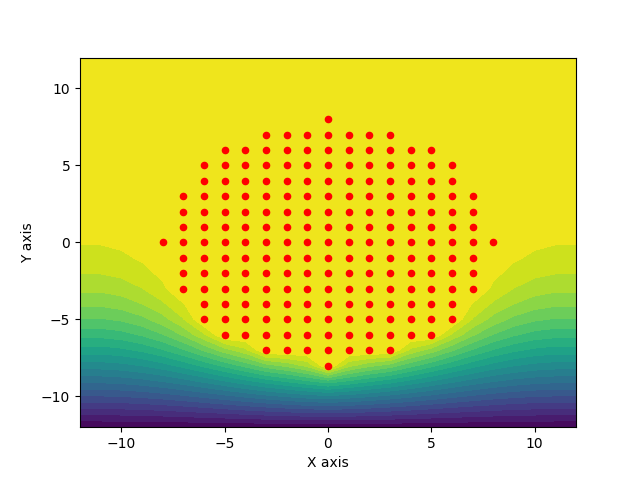
\includegraphics[scale=0.9,width=\linewidth]{fig1.png} 
    \caption{Figure 1}
    \label{fig:my_label}
\end{subfigure}
\begin{subfigure}{0.55\textwidth}
    \centering
    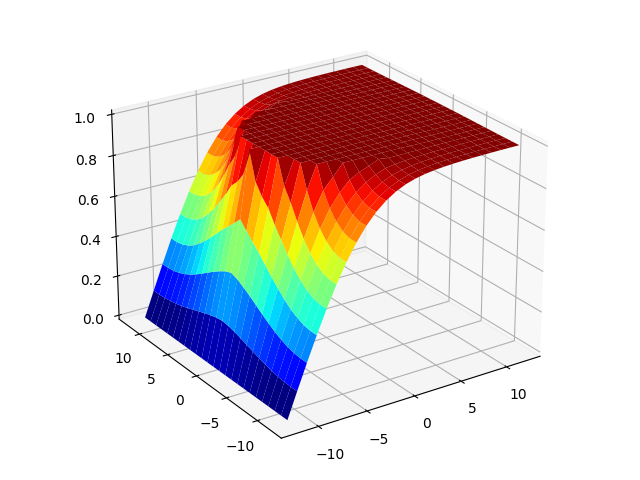
\includegraphics[scale=0.9,width=\linewidth]{fig5.png} 
    \caption{Figure 2}
    \label{fig:image2}
\end{subfigure}


\end{figure}


\subsection{Fitting the Error as a Function of no. of Iterations.}
We fit the Error into the function,

\begin{equation}\label{eq:4}
log(y) = log(A)+Bx
\end{equation}
Where $y$ is the error, $A$ and $B$ are parameters to be computed and x is the Iteration Number. We find the parameters with the help of the function {\fontfamily{cmss}\selectfont
'lstsq()'
}. With the predicted function, we plot the errors, along with the real error as a function of the number of Iterations.  We also plot the semilog and loglog plots of the real Error. The below code accomplishes the above tasks.
\\
\\
\lstinputlisting[language = python]{code2.py}
\begin{figure}[h!]

\begin{subfigure}{0.55\textwidth}
    
    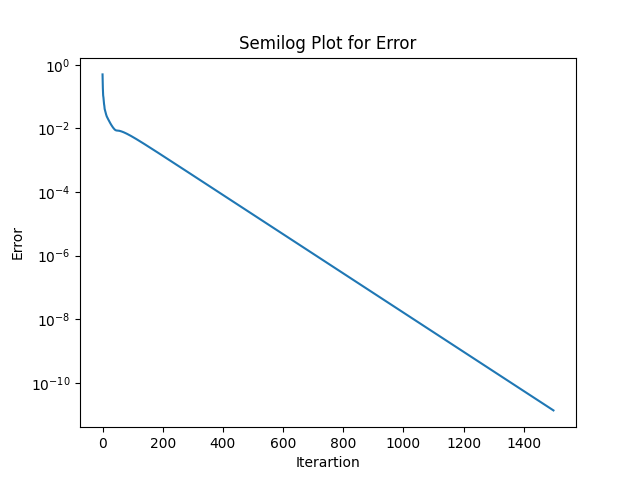
\includegraphics[scale=0.9,width=\linewidth]{fig2.png} 
    \caption{Figure 5}
    \label{fig:my_label}
\end{subfigure}
\begin{subfigure}{0.55\textwidth}
   
    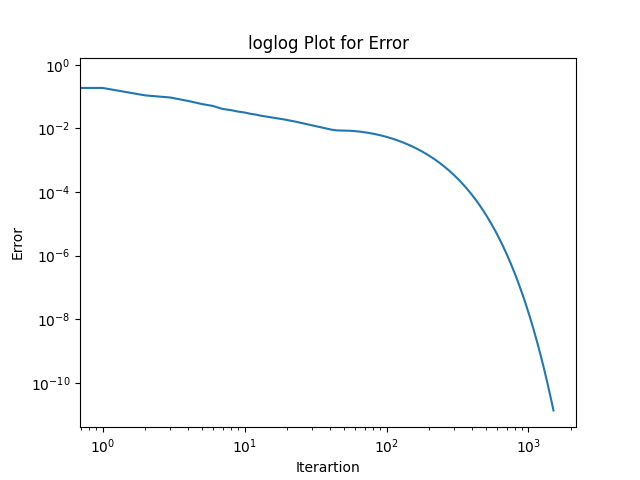
\includegraphics[scale=0.9,width=\linewidth]{fig3.png} 
    \caption{Figure 6}
    \label{fig:image2}
\end{subfigure}
\end{figure}
\begin{figure}[h!]
    \centering
    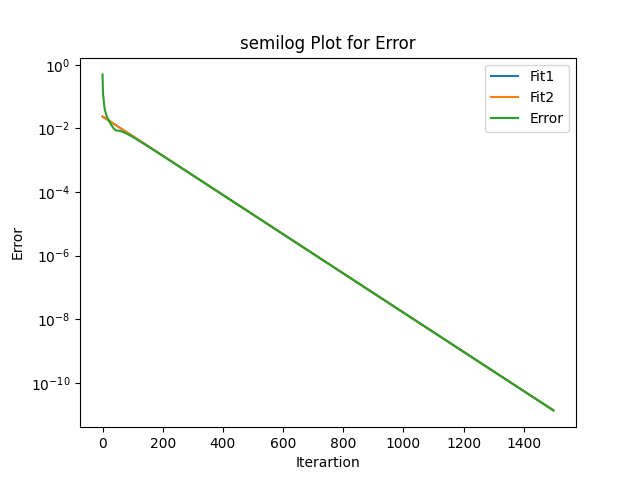
\includegraphics[scale=0.75]{fig4.png} 
    \caption{}
    \label{fig:my_label}
\end{figure}
\vspace{100mm}
\vspace{100mm}

\subsection{Finding and Vector Plotting the Currents}
The Currents are found by Computing the gradient of the Potential Function. Then using the function quiver, the Vector plots of the Current are plotted. The below code accomplishes the above tasks,
\noindent
\vspace{5mm}
\lstinputlisting[language = python]{code3.py}
\begin{figure}[h!]
    \centering
    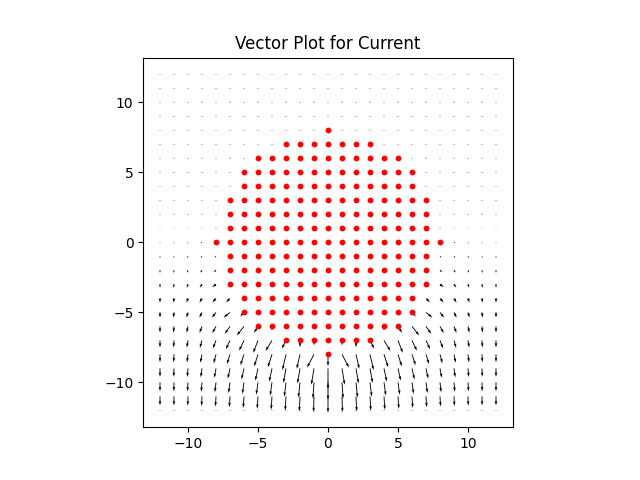
\includegraphics[scale=0.68]{fig6.png} 
    \caption{}
    \label{fig:my_label}
\end{figure}
\section{Conclusion}
The Resistor problem is solved using the Laplace equation. Contour and 3D plots for the potential Function are plotted. The max error is computed and semilog and loglog plots are plotted. We find the current densities. The heat produced is maximum where there the current is maximum


\end{document}

